%----------------------------------------------------------------------------------------
%	PACKAGES AND OTHER DOCUMENT CONFIGURATIONS
%----------------------------------------------------------------------------------------

\documentclass[11pt]{article}

%----------------------------------------------------------------------------------------
%	PACKAGES AND OTHER DOCUMENT CONFIGURATIONS
%----------------------------------------------------------------------------------------

\usepackage{lastpage} % Required to determine the last page number for the footer

\usepackage{multicol}

\usepackage{nth}

\usepackage{graphicx} % Required to insert images

\setlength\parindent{0pt} % Removes all indentation from paragraphs

\usepackage[most]{tcolorbox} % Required for boxes that split across pages

\usepackage{booktabs} % Required for better horizontal rules in tables

\usepackage{listings} % Required for insertion of code

\usepackage{etoolbox} % Required for if statements

%----------------------------------------------------------------------------------------
%	MARGINS
%----------------------------------------------------------------------------------------

\usepackage{geometry} % Required for adjusting page dimensions and margins

\geometry{
	paper=a4paper, % Change to letterpaper for US letter
	top=3cm, % Top margin
	bottom=3cm, % Bottom margin
	left=2.5cm, % Left margin
	right=2.5cm, % Right margin
	headheight=14pt, % Header height
	footskip=1.4cm, % Space from the bottom margin to the baseline of the footer
	headsep=1.2cm, % Space from the top margin to the baseline of the header
	%showframe, % Uncomment to show how the type block is set on the page
}

%----------------------------------------------------------------------------------------
%	FONT
%----------------------------------------------------------------------------------------

\usepackage[utf8]{inputenc} % Required for inputting international characters
\usepackage[T1]{fontenc} % Output font encoding for international characters

\usepackage[sfdefault,light]{roboto} % Use the Roboto font

%----------------------------------------------------------------------------------------
%	HEADERS AND FOOTERS
%----------------------------------------------------------------------------------------

\usepackage{fancyhdr} % Required for customising headers and footers

\pagestyle{fancy} % Enable custom headers and footers

\lhead{\assignmentTitle} % Left header; output the instructor in brackets if one was set
\chead{} % Centre header
\rhead{\assignmentAuthorName} % Right header; output the author name if one was set, otherwise the due date if that was set

\lfoot{} % Left footer
\cfoot{\small Page\ \thepage\ of\ \pageref{LastPage}} % Centre footer
\rfoot{} % Right footer

\renewcommand\headrulewidth{0.5pt} % Thickness of the header rule

%----------------------------------------------------------------------------------------
%	MODIFY SECTION STYLES
%----------------------------------------------------------------------------------------

\usepackage{titlesec} % Required for modifying sections

%------------------------------------------------
% Section

\titleformat
{\section} % Section type being modified
[block] % Shape type, can be: hang, block, display, runin, leftmargin, rightmargin, drop, wrap, frame
{\Large\bfseries} % Format of the whole section
{\assignmentQuestionName~\thesection} % Format of the section label
{6pt} % Space between the title and label
{} % Code before the label

\titlespacing{\section}{0pt}{0.5\baselineskip}{0.5\baselineskip} % Spacing around section titles, the order is: left, before and after

%------------------------------------------------
% Subsection

\titleformat
{\subsection} % Section type being modified
[block] % Shape type, can be: hang, block, display, runin, leftmargin, rightmargin, drop, wrap, frame
{\itshape} % Format of the whole section
{(\alph{subsection})} % Format of the section label
{4pt} % Space between the title and label
{} % Code before the label

\titlespacing{\subsection}{0pt}{0.5\baselineskip}{0.5\baselineskip} % Spacing around section titles, the order is: left, before and after

\renewcommand\thesubsection{(\alph{subsection})}

%----------------------------------------------------------------------------------------
%	CUSTOM QUESTION COMMANDS/ENVIRONMENTS
%----------------------------------------------------------------------------------------

% Environment to be used for each question in the assignment
\newenvironment{question}{
	\vspace{0.5\baselineskip} % Whitespace before the question
	\section{} % Blank section title (e.g. just Question 2)
	\lfoot{\small\itshape\assignmentQuestionName~\thesection~continued on next page\ldots} % Set the left footer to state the question continues on the next page, this is reset to nothing if it doesn't (below)
}{
	\lfoot{} % Reset the left footer to nothing if the current question does not continue on the next page
}

%------------------------------------------------

% Environment for subquestions, takes 1 argument - the name of the section
\newenvironment{subquestion}[1]{
	\subsection{#1}
}{
}

%------------------------------------------------

% Command to print a question sentence
\newcommand{\questiontext}[1]{
	\textbf{#1}
	\vspace{0.5\baselineskip} % Whitespace afterwards
}

%------------------------------------------------

% Command to print a box that breaks across pages with the question answer
\newcommand{\answer}[1]{
	\begin{tcolorbox}[breakable, enhanced]
		#1
	\end{tcolorbox}
}

%------------------------------------------------

% Command to print a box that breaks across pages with the space for a student to answer
\newcommand{\answerbox}[1]{
	\begin{tcolorbox}[breakable, enhanced]
		\vphantom{L}\vspace{\numexpr #1-1\relax\baselineskip} % \vphantom{L} to provide a typesetting strut with a height for the line, \numexpr to subtract user input by 1 to make it 0-based as this command is
	\end{tcolorbox}
}

%------------------------------------------------

% Command to print an assignment section title to split an assignment into major parts
\newcommand{\assignmentSection}[1]{
	{
		\centering % Centre the section title
		\vspace{2\baselineskip} % Whitespace before the entire section title
		
		\rule{0.8\textwidth}{0.5pt} % Horizontal rule
		
		\vspace{0.75\baselineskip} % Whitespace before the section title
		{\LARGE \MakeUppercase{#1}} % Section title, forced to be uppercase
		
		\rule{0.8\textwidth}{0.5pt} % Horizontal rule
		
		\vspace{\baselineskip} % Whitespace after the entire section title
	}
}

%----------------------------------------------------------------------------------------
%	TITLE PAGE
%----------------------------------------------------------------------------------------

\author{\textbf{\assignmentAuthorName}} % Set the default title page author field
\date{} % Don't use the default title page date field

\title{
	\thispagestyle{empty} % Suppress headers and footers
	\vspace{0.2\textheight} % Whitespace before the title
	\textbf{\assignmentTitle}\\[-4pt]
	\ifdef{\assignmentDueDate}{{\small Due\ on\ \assignmentDueDate}\\}{} % If a due date is supplied, output it
	\ifdef{\assignmentClassInstructor}{{\large \textit{\assignmentClassInstructor}}}{} % If an instructor is supplied, output it
	\vspace{0.32\textheight} % Whitespace before the author name
}
 % Include the file specifying the document structure and custom commands

%----------------------------------------------------------------------------------------
%	ASSIGNMENT INFORMATION
%----------------------------------------------------------------------------------------

% Required
\newcommand{\assignmentQuestionName}{Part} % The word to be used as a prefix to question numbers; example alternatives: Problem, Exercise
\newcommand{\assignmentClass}{} % Course/class
\newcommand{\assignmentTitle}{The Origins of the French Intervention in the Russian Civil War — Handout} % Assignment title or name
\newcommand{\assignmentAuthorName}{Michael Brodskiy} % Student name



\begin{document}


\maketitle % Print the title page

\thispagestyle{empty} % Suppress headers and footers on the title page

\newpage

\begin{multicols}{2}

\begin{center}
  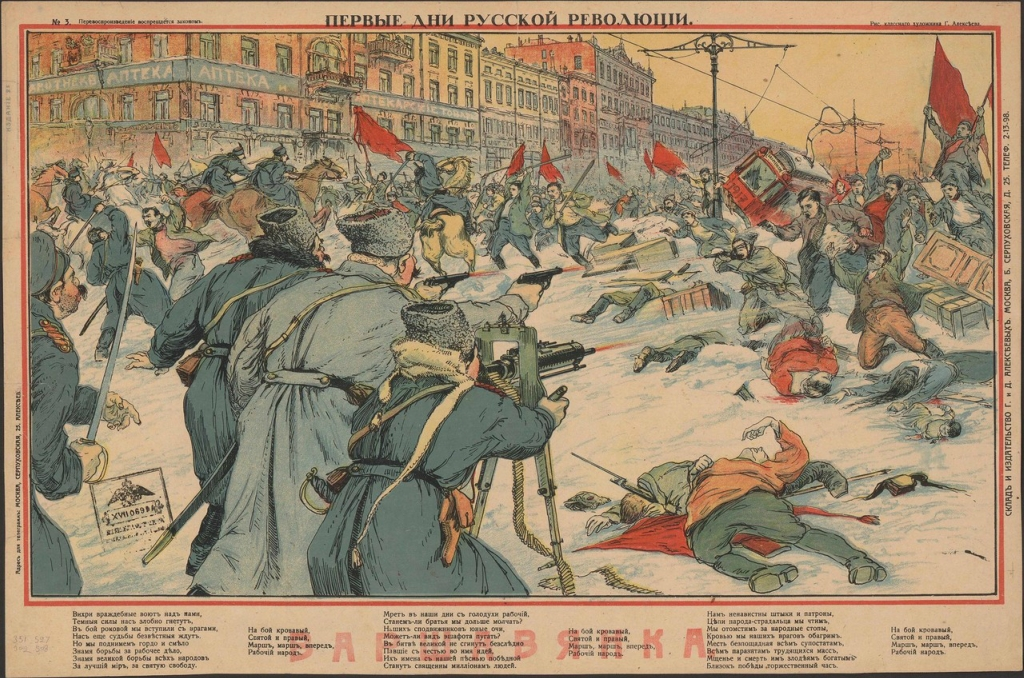
\includegraphics[width=0.95\columnwidth]{images/FirstDays.jpg}
\end{center}
\begin{center}
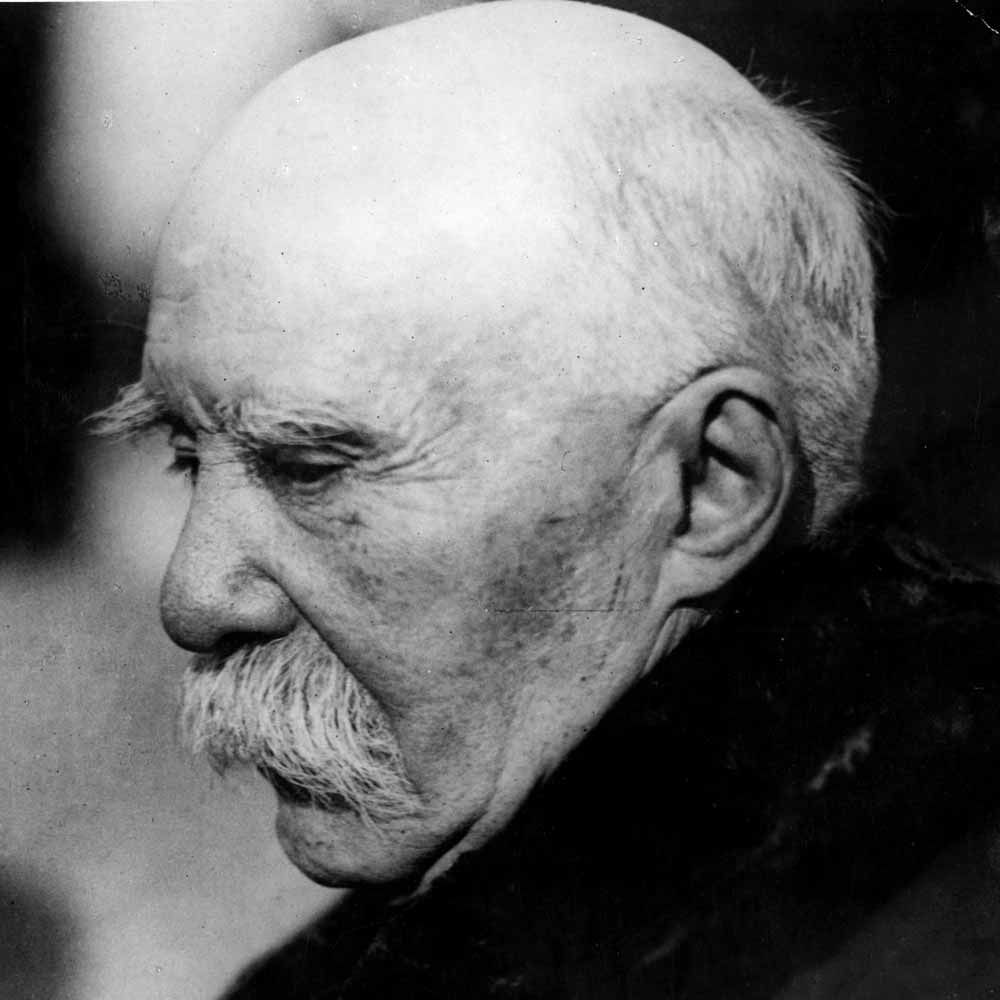
\includegraphics[width=.475\columnwidth]{images/Clemenceau.jpg}
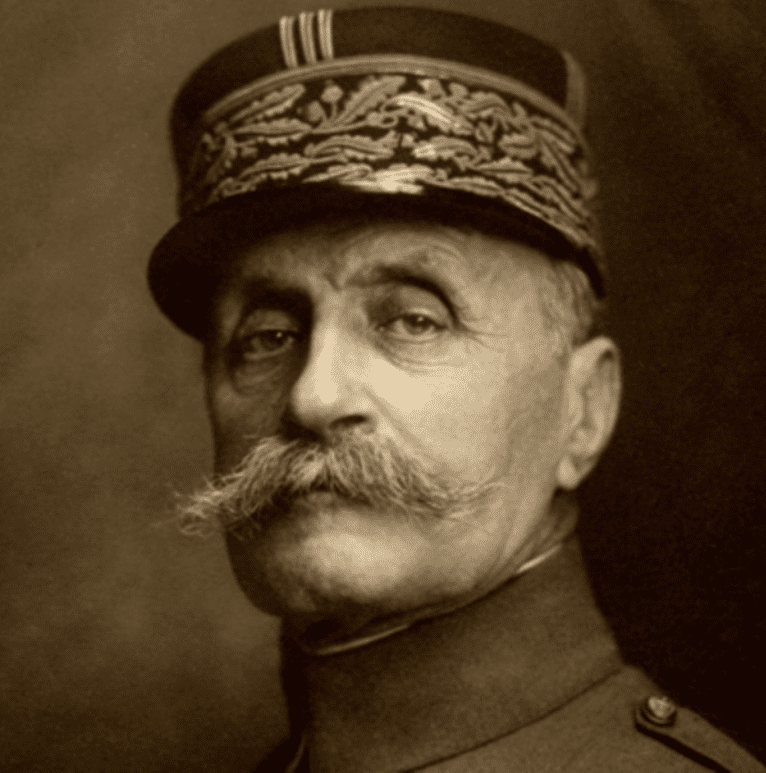
\includegraphics[width=.475\columnwidth]{images/Foch.png}
\end{center}

\answer{\begin{center}\underline{Major French Players} \end{center}\vspace{-10pt}\begin{itemize} \item Quai d'Orsay — Ministry for Europe and Foreign Affairs \begin{itemize} \vspace{-5pt} \item Philippe Berthelot — Deputy Director \vspace{-5pt} \end{itemize} \item Georges Clemenceau — Prime Minister \vspace{-5pt} \item Henri Albert Niessel — General of the Russian Mission \vspace{-5pt} \item Ferdinand Foch — Chief of General Staff \vspace{-7pt} \item Stephen Pichon — Foreign Minister \vspace{-20pt} \item Joseph Noulens — Ambassador to Russia \end{itemize}}

\end{multicols}

\vspace{-25pt}

\begin{multicols}{2}

  \answer{\begin{itemize} \item Initially, the policy was “to hasten the end of the anarchy in Russia and to facilitate the reestablishment of order and a legal government." — Stephen Pichon \begin{itemize} \item Ukraine was used as a leverage point (by recognizing its independence) \end{itemize} \end{itemize}}
  \vspace{-12pt}
  \answer{\begin{itemize} \item Brest-Litovsk talks, beginning in December 1917, worried the French  \item Military Intelligence suggested rapprochement \item Limited ties with Bolsheviks were approved around mid-February \item Tried to appease Bolsheviks \begin{itemize} \item Ties improved, in early March Niessel corresponded with Trotsky regularly \end{itemize} \end{itemize}}

  \begin{center}
    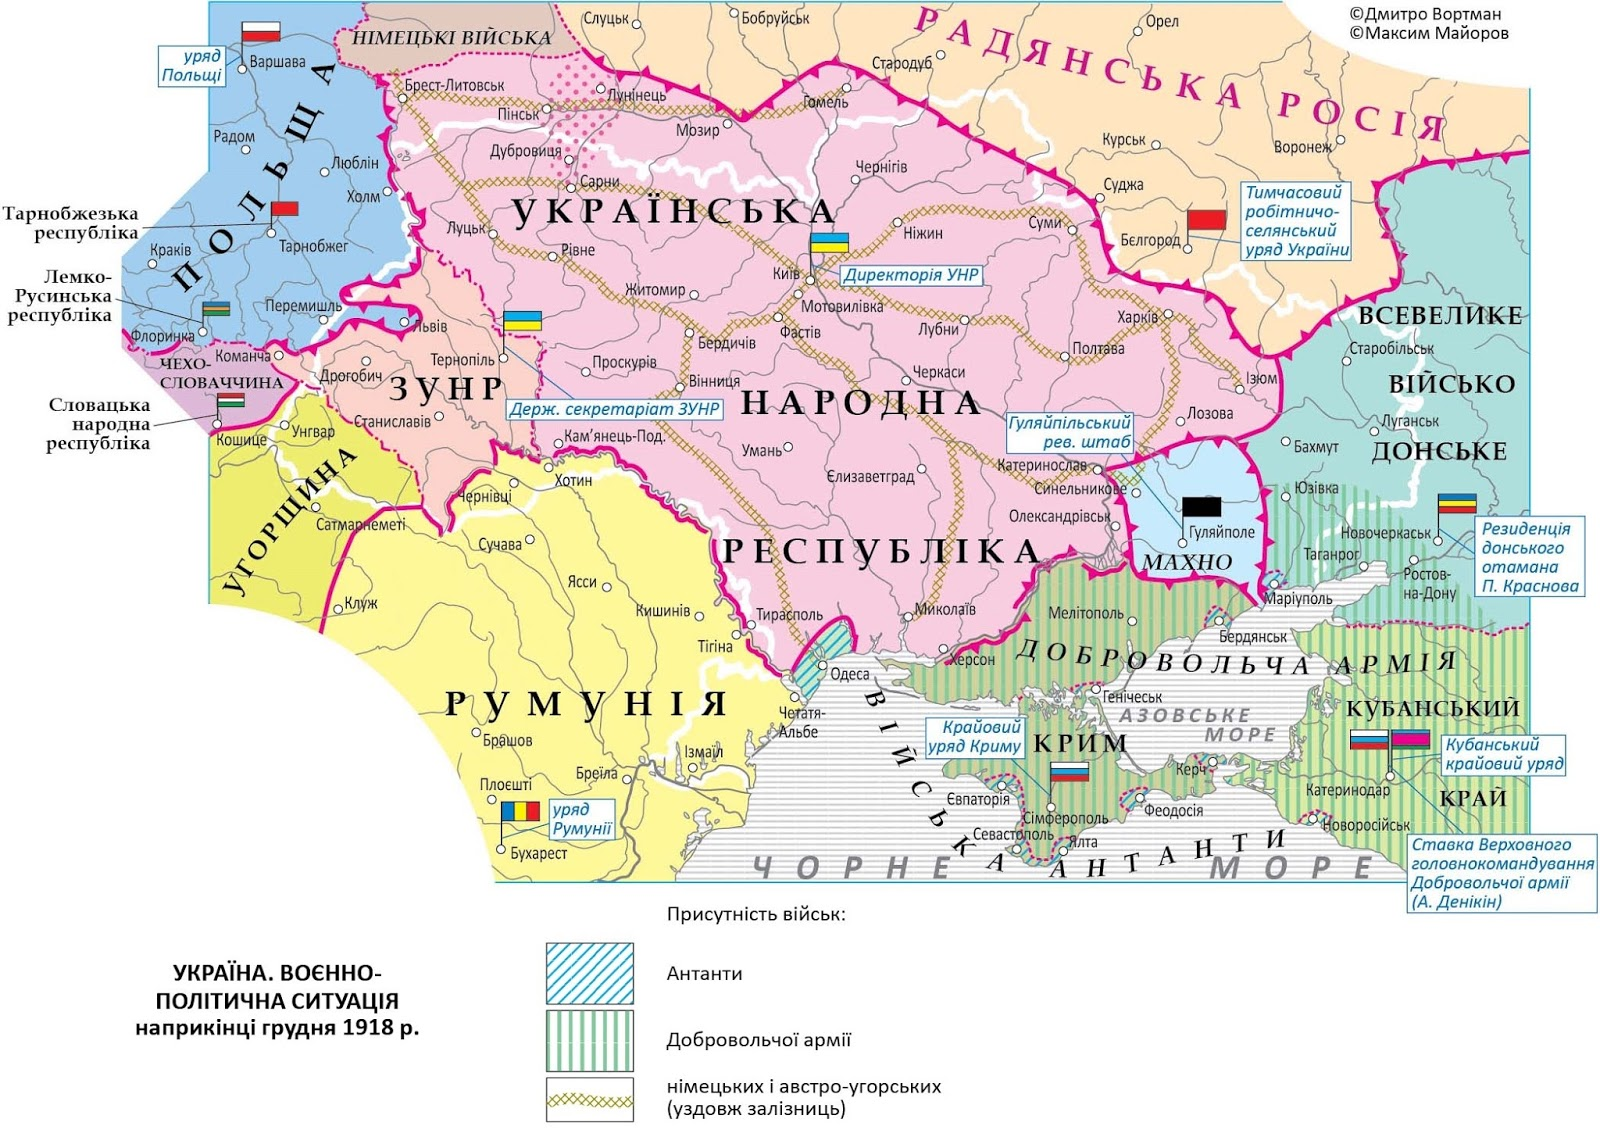
\includegraphics[width=.95\columnwidth]{images/Ukraine.png}
  \end{center}
  \begin{center}
    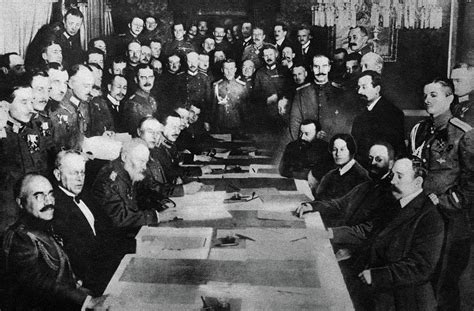
\includegraphics[width=.95\columnwidth]{images/Brest-Litovsk.jpeg}
  \end{center}

\end{multicols}

\vspace{-25pt}

\begin{multicols}{2}

  \answer{\begin{itemize} \item On March \nth{20}, after becoming the Military Leader, Trotsky requested military support \vspace{-10pt} \begin{itemize} \item Guillaum Lavergne, who replaced Niessel, approved  \end{itemize} \end{itemize}}

  \answer{\begin{itemize} \item Ministry of War offered limited support to Lavergne \item Noulens asked to reanalyze situation, proposed a break in ties \vspace{3.5pt} \end{itemize}}

\end{multicols}

\assignmentSection{Reversal in Policy}

\vspace{-10pt}

\begin{multicols}{2}

\begin{center}
  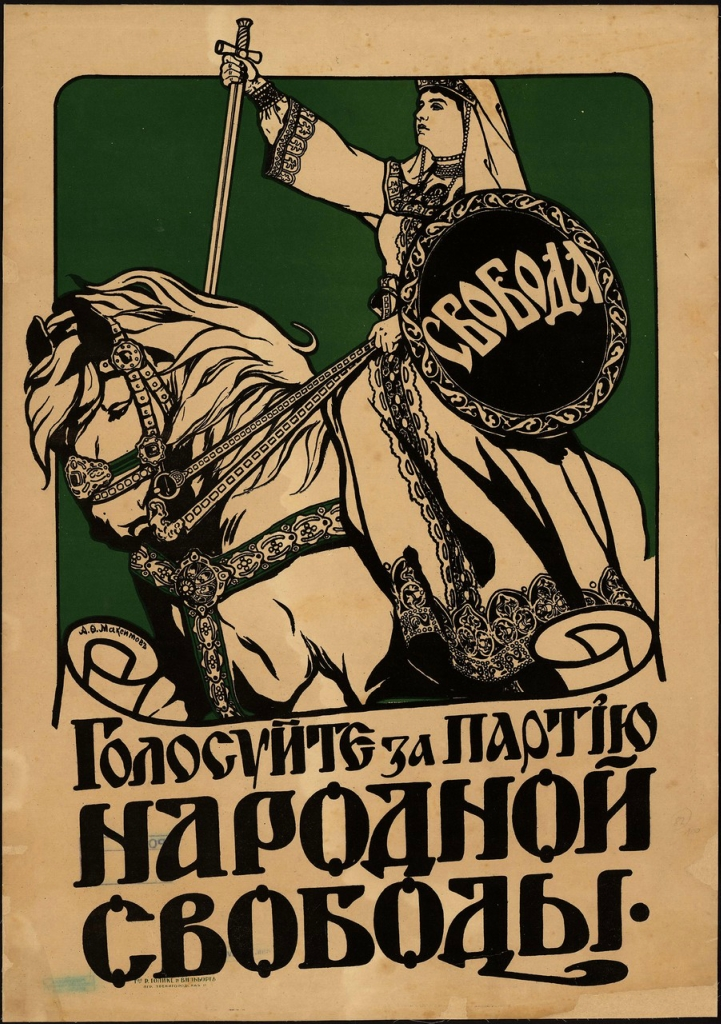
\includegraphics[width=.475\columnwidth]{images/Freedom.png}
  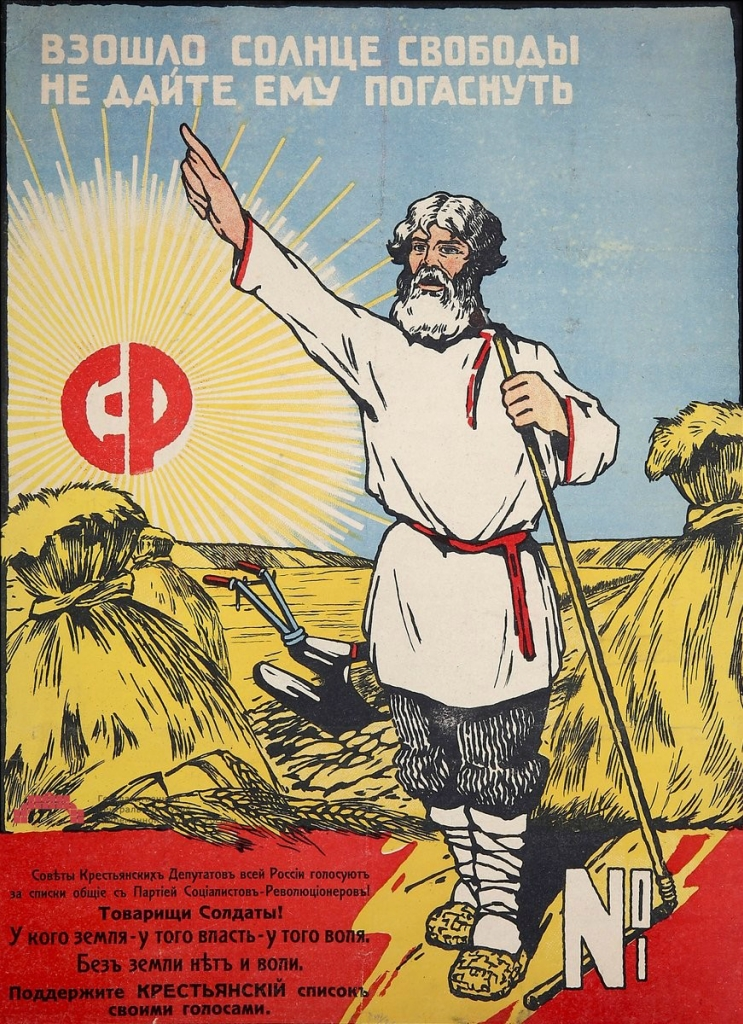
\includegraphics[width=.475\columnwidth]{images/Sun.png}
\end{center}

\answer{\begin{itemize} \item Quai d'Orsay began to worry more about spread of \textit{guerre sociale} \item Policy began to reverse, relations deteriorated \item First, on April \nth{5}, Lavergne was ``given a certain freedom of action'' \item Next, on April \nth{9}, Noulens requested control over Lavergne \end{itemize}}

\end{multicols}

\begin{multicols}{2}

  \answer{\begin{itemize} \item Noulens had his request approved on April \nth{16} \item Thus, policy reversal took place from April \nth{5}—\nth{16} \item Foch's resignation played a main role in allowing policy reversal \begin{itemize} \item Historians believe this because he signed most pro-rapprochement documents  \end{itemize} \end{itemize}}

\begin{center}
  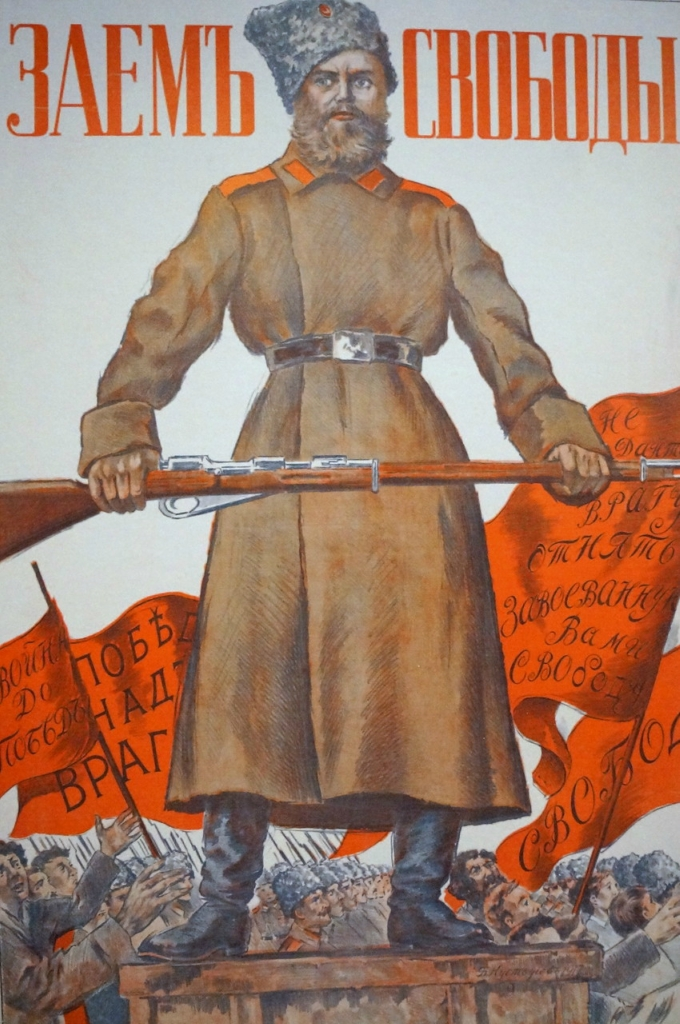
\includegraphics[width=.475\columnwidth]{images/Zaem.png}
  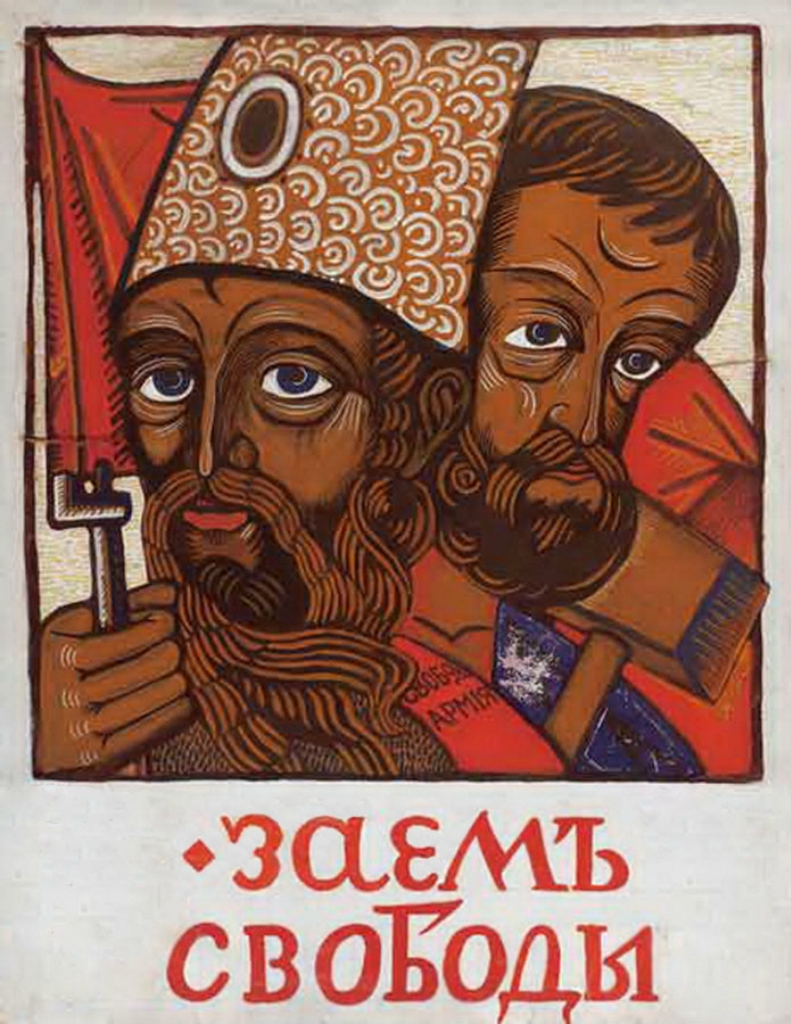
\includegraphics[width=.475\columnwidth]{images/Zaem.jpg}
\end{center}

\end{multicols}

\vspace{-40pt}

\assignmentSection{In Conclusion \ldots }

\vspace{-10pt}

\begin{multicols}{2}

  \begin{center}
    \includegraphics[width=.475\columnwidth]{images/Anarchy.jpg} 
    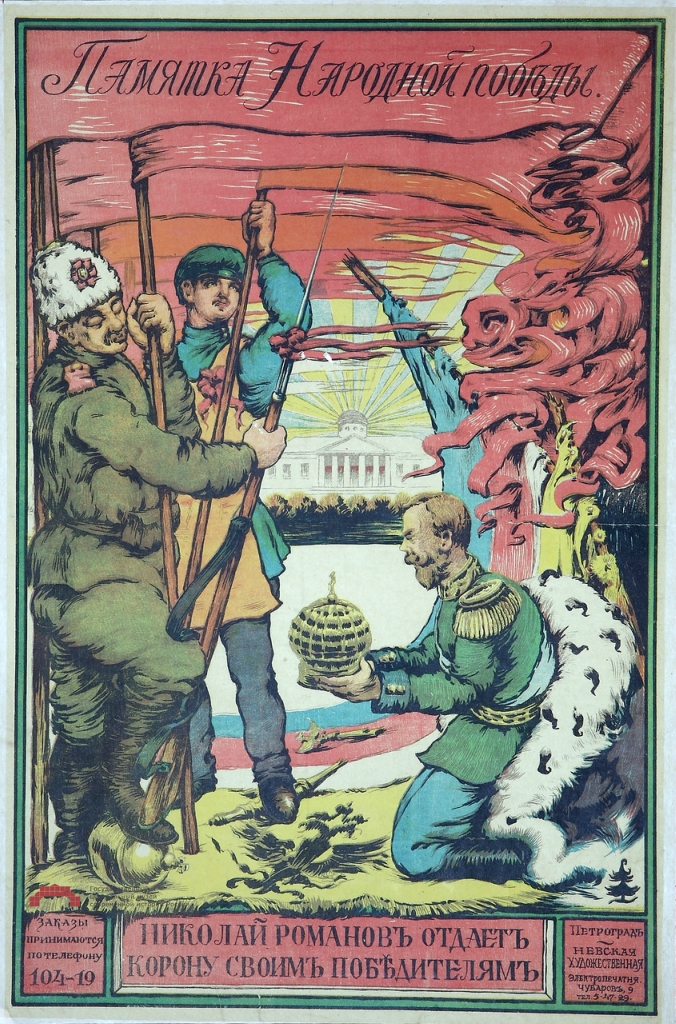
\includegraphics[width=.475\columnwidth]{images/King.jpg} 
  \end{center}

  \answer{\begin{itemize} \item French disorganization contributed to reversal \begin{itemize} \item Many players, with differing perspectives \end{itemize} \item Lots of uncertainty \begin{itemize} \item Marxist revolution never-before-seen \item Many factors to consider in analysis  \end{itemize} \item This makes either historian perspective partially true \end{itemize}}

\end{multicols}

\end{document}
